\documentclass{beamer}
\usepackage[russian]{babel}
\usetheme{metropolis}

\usepackage{amsthm}
\setbeamertemplate{theorems}[numbered]

\setbeamercolor{block title}{use=structure,fg=white,bg=gray!75!black}
\setbeamercolor{block body}{use=structure,fg=black,bg=gray!20!white}

\usepackage[T2A]{fontenc}
\usepackage[utf8]{inputenc}

\usepackage{hyphenat}
\usepackage{amsmath}
\usepackage{graphicx}

\AtBeginEnvironment{proof}{\renewcommand{\qedsymbol}{}}{}{}

\title{
Микроэкономика-I
}
\author{
Павел Андреянов, PhD
}

\begin{document}

\maketitle

\begin{frame}{План лекции}

\begin{itemize}
  \item Часть 1. Фестиваль свободного творчества по применению теоремы об огибающей. Модели Леонтьева
  \item Часть 2. Абстрактные технологические множества. Сложение треугольников.
\end{itemize}


\end{frame}

\section{Три задачи производителя}

\begin{frame}{Три задачи производителя}

Напомню, что у нас есть три задачи оптимизации в теории производителя

\begin{itemize}
  \item минимизация издержек при заданном выпуске $y$
  $$ p x \to \min_x, \quad F(x) \geqslant y $$
  \item следующая за ней максимизация прибыли
  $$ q y - TC(y|p) \to \max_y$$
  \item максимизация прибыли в один шаг
  $$ q y - p x \to \max_{x,y}, \quad F(x) \geqslant y$$
\end{itemize}

Тут $(\vec x, \vec y)$ это факторы и конечные товары, а $(\vec p, \vec q)$ это их соответствующие цены.

\end{frame}

\section{Минимизация издержек}

\begin{frame}{Минимизация издержек}

Напомню, что минимизация издержек создает функцию спроса на факторы производства:

\begin{itemize}
  \item если ваша фирма строительная, то она создает спрос на кирпичи и цемент
  \item если ваша фирма ресторан, то она создает спрос на ингредиенты
  \item если ваша фирма школа, она создает спрос на труд (преподавателей)
\end{itemize}

Вопрос: является ли спрос монотонным по собственным ценам? Не может ли у нас случиться как с парадоксом Гиффена?

\end{frame}

\begin{frame}{Минимизация издержек}

$$ p x \to \min_x, \quad F(x) \geqslant y $$

где $F(x)$ - функция описывающая превращение факторов $x$ в конечный товар $y$

Ответим сначала на два вопроса:

\begin{itemize}
  \item Что является координатой максимума?
  \item Что является значением в максимуме?
  \item Что является пространством параметров?
\end{itemize}

Подсказка: это функции от параметров задачи $p, y$.

\end{frame}

\begin{frame}{Минимизация издержек}

Правильные ответы

\begin{itemize}
  \item координата максимума: условный спрос $\tilde x(p| y)$
  \item значение в максимуме: функция издержек $TC(p| y)$
  \item пространство параметров: $p, y$
\end{itemize}

Новое обозначение <<вертикальная палка>> означает <<условно на что то>>, она отделяет второстепенные параметры функции от первостепенных. Для каждой функции они свои.

\end{frame}

\begin{frame}{Минимизация издержек}

Теперь применим теорему об огибающей.
$$ p x \to \min_x, \quad F(x) \geqslant y $$

Заметим, что в пространстве параметра $p$ опорные функции - линейны. И мы ищем минимум. Значит у нас получается нижняя огибающая линейного семейства, она вогнутая. 

Соответственно, функция издержек вогнута по ценам факторов (нарисуй картинку). Более того, наклон функции издержек $TC(p|y)$ по цене равен просто оптимальному $\tilde x(p|y)$.

\end{frame}

\begin{frame}{Минимизация издержек}

Итак, функция издержек вогнута по ценам факторов, а наклон функции издержек $TC(p|y)$ по цене равен просто оптимальному $\tilde x(p|y)$.

Поскольку у вогнутой функции в Гессиане, грубо говоря, на диагонали стоят отрицательные числа, получается что условный спрос $\tilde x(p|y)$ всегда убывает по собственным ценам.

\alert{В теории производителя не бывает парадоксов Гиффена}.

\end{frame}

\section{Максимизация прибыли}

\begin{frame}{Максимизация прибыли}

Напомню, что максимизация прибыли создает функцию предложения конечного товара:

\begin{itemize}
  \item если ваша фирма строительная, то она создает предложение квартир и домов
  \item если ваша фирма ресторан, то она создает предложение обедов
  \item если ваша фирма школа, она создает предложение образовательных услуг
\end{itemize}

Вопрос: является ли предложение монотонным по собственным ценам?
\end{frame}

\begin{frame}{Максимизация прибыли}

$$ q y - TC(y| p) \to \max_y$$

Ответим сначала на три вопроса:

\begin{itemize}
  \item Что является координатой максимума?
  \item Что является значением в максимуме?
  \item Что является пространством параметров?
\end{itemize}

Подсказка: это функции от параметров задачи $q, p$.

\end{frame}

\begin{frame}{Максимизация прибыли}

Правильные ответы

\begin{itemize}
  \item координата максимума: предложение $y (q| p)$
  \item значение в максимуме: прибыль $\pi(q| p)$
  \item пространство параметров: $q, p$
\end{itemize}

напомню что $q$ это цена конечного товара, а $p$ это цена фактора.

\end{frame}

\begin{frame}{Максимизация прибыли}

Теперь применим теорему об огибающей.
$$ q y - TC(y| p) \to \max_y$$
Заметим, что в пространстве параметра $q$ опорные функции - линейны. И мы ищем максимум. Значит у нас получается верхняя огибающая линейного семейства, она выпукла. 

Соответственно, функция прибыли выпукла по ценам конечных товаров (нарисуй картинку). Более того, наклон функции прибыли $\pi(q|p)$ по цене $q$ равен просто оптимальному $y(q|p)$.
\end{frame}

\begin{frame}{Максимизация прибыли}

Итак, функция прибыли выпукла по ценам конечных товаров, а наклон функции прибыли по цене равен просто оптимальному уровню производства.

Поскольку у выпуклой функции в Гессиане, грубо говоря, на диагонали стоят положительные числа, получается что \alert{предложение всегда возрастает по собственным ценам}.

\end{frame}

\section{Максимизация прибыли вош.}

\begin{frame}{Максимизация прибыли вош}

Напомню, что максимизация прибыли создает функцию предложения конечного товара и спрос на факторы:

\begin{itemize}
  \item если ваша фирма строительная, то она создает предложение квартир и домов и спрос на кирпич и цемент
  \item если ваша фирма ресторан, то она создает предложение обедов и спрос на ингридиенты
  \item если ваша фирма школа, она создает предложение образовательных услуг и спрос на труд преподавателей
\end{itemize}

Вопрос: является ли спрос и предложение монотонным по (соответствующим) собственным ценам?
\end{frame}

\begin{frame}{Максимизация прибыли вош}

$$ q y - p x \to \max_{x,y}, \quad F(x) \geqslant y$$

Ответим сначала на три вопроса:

\begin{itemize}
  \item Что является координатой максимума?
  \item Что является значением в максимуме?
  \item Что является пространством параметров?
\end{itemize}

Подсказка: это функции от параметров задачи $q, p$.

\end{frame}

\begin{frame}{Максимизация прибыли вош}

Правильные ответы

\begin{itemize}
  \item координата максимума: спрос и предложение $x(p|q), y(q|p)$
  \item значение в максимуме: прибыль $\pi(p, q)$
  \item пространство параметров: $p, q$
\end{itemize}

напомню что $q$ это цена конечного товара, а $p$ это цена фактора.

\end{frame}

\begin{frame}{Максимизация прибыли вош}

Теперь применим теорему об огибающей.
$$ q y - p x \to \max_{x,y}, \quad F(x) \geqslant y$$
Заметим, что в пространстве параметров $p,q$ опорные функции - линейны. И мы ищем максимум. Значит у нас получается верхняя огибающая линейного семейства, она выпукла. 

Соответственно, функция прибыли выпукла по ценам вообще всех товаров. Более того, наклон функции прибыли $\pi(p, q)$ по цене $p$ равен просто оптимальному $-x$ а по цене $q$ просто оптимальному $y$.
\end{frame}

\begin{frame}{Максимизация прибыли вош}

Итак, функция прибыли выпукла по вообще всем ценам $(p,q)$, а наклон функции прибыли по цене равен просто оптимальному $(-x,y)$.

Поскольку у выпуклой функции в Гессиане, грубо говоря, на диагонали стоят положительные числа, получается что $-x$ возрастает по $p$, а $y$ возрастает по $q$. 

Что и требовалось доказать.

\end{frame}

\section{А что если фирма монополист?}

\begin{frame}{А что если фирма монополист?}

Напомню, что глядя на цены конечных товаров $q$, фирма цено-получатель выбирает уровень производства $y$ так чтобы $$q = MC(y).$$ 

А фирма монополист выбирает согласно правилу обратной эластичности
$$ \frac{q(y)-MC(y)}{q(y)} = - \frac{1}{\varepsilon}.$$

При этом, вывод самой функции издержек TC(y) не зависит от того, монополист фирма или цено-получатель, это просто эффективное расходование ресурсов, поверьте мне.

\end{frame}

\section{Модели Леонтьева}

\begin{frame}{Модели Леонтьева}
\begin{columns}
\begin{column}{0.5\textwidth}
   \alert{Василий Леонтьев} американский экономист российского происхождения, \alert{создатель теории межотраслевого анализа}. 
   
   \medskip
   
   После эмиграции и начала второй мировой войны работал консультантом по экономическому планированию для военно-воздушных сил США.
   
\end{column}
\begin{column}{0.5\textwidth}  %%<--- here
    \begin{center}
     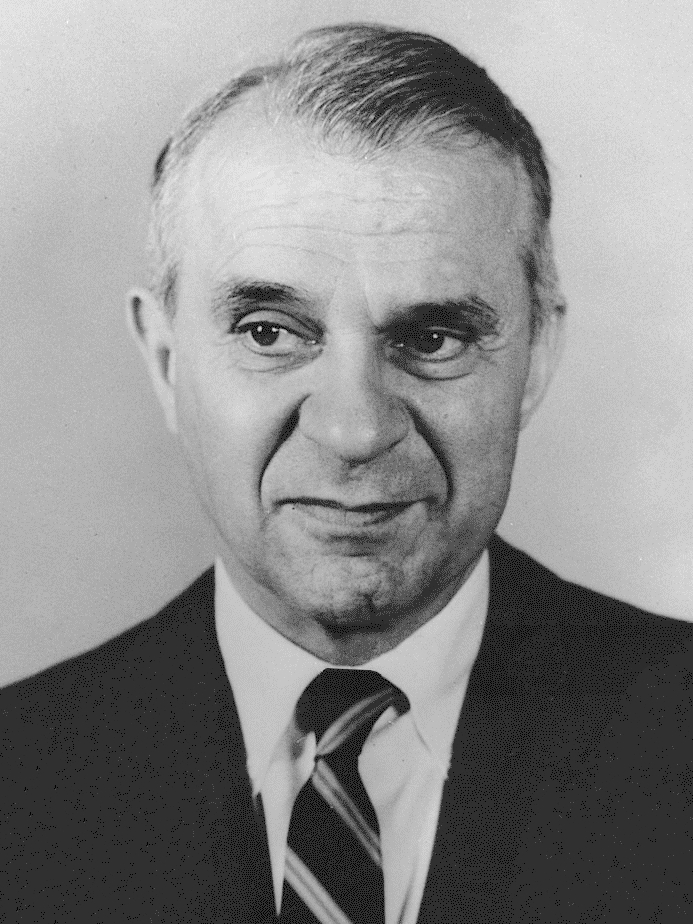
\includegraphics[width=1\textwidth]{leont}
     \end{center}
\end{column}
\end{columns}
\end{frame}

\begin{frame}{Модели Леонтьева}
Итак, модели Леонтьева построены на следующем предположении:

\begin{itemize}
  \item фирма потребляет факторы $\vec x$ и только один конечный товар
  \item технология описывается функцией минимум
$$ \min(\frac{x_1}{a_1}, \ldots, \frac{x_n}{a_n}).$$
\end{itemize}
То есть, для производства одной единицы конечного товара, требуется $a_1, \ldots, a_n$ единиц соответствующих факторов. Это хорошо подходит для моделирования впк страны.
\end{frame}

\begin{frame}{Модели Леонтьева}
Можно заметить, что

\begin{itemize}
  \item независимо от цен, факторы потребляются в фиксированных пропорциях
  \item функция издержек линейна по уровню производства
  \item прибыль линейна по по уровню производства
\end{itemize}

Это значит, что прибыль особо не помаксимизируешь, оптимальный $y$ уйдет в бесконечность. Но зато это хорошо подходит для плановой экономики, скажем, СССР.
 
\end{frame}

\begin{frame}{Модели Леонтьева}

Раз экономика плановая, забудем про цены ненадолго.

\begin{itemize}
  \item пусть есть $n$ отраслей (заводов)
  \item они производят $n$ видов продукции (товаров)
  \item каждый завод $i$ производит $x_i$ из $\vec x = (x_1, \ldots, x_n)$
  \item эффективное производство можно записать как
      $$ x_i = a_{i1} x_1 + a_{i2} x_2 + \ldots + a_{in} x_n.$$
\end{itemize}

Часть из них может быть прямо ресурс, как уголь и сталь.

Часть из них может быть промежуточным товаром, как гвозди.

Часть из них может быть каким-то понятным конечным товаром, например, легковым автомобилем или табуреткой.
\end{frame}

\begin{frame}{Модели Леонтьева}
Запишем все при помощи матрицы $A = \{a_{ij}\}$
  $$x - y = Ax$$
где $x$ это общий (валовый) спрос а $y$ это конечный (чистый). 

Разница между двумя спросами $x - y$ это те факторы которые были потреблены в эффективном производственном процессе. 

Они то и описываются линейными уравнениями $Ax$.
\end{frame}

\begin{frame}{Модели Леонтьева}
Наконец, обратим систему
  $$x = (I-A)^{-1} y$$
и мы получим связь между количеством чистого ($y$) и валового ($x$) товара.

\end{frame}

\begin{frame}{Модели Леонтьева}
Рассмотрим пример с 2 отраслями: производство угля и стали.

Уголь требуется для производства стали, а некоторое количество стали — в виде инструментов — для добычи угля. 

Предположим, что условия таковы: для производства 1 т стали нужно 3 т угля, а для 1 т угля — .1 т стали.

\end{frame}

\begin{frame}{Модели Леонтьева}

Пусть $y = (100, 100)$ это желаемое количество стали и угля.
$$
x - y = A x, \quad A =\begin{pmatrix}
  0 & 3\\
  .1 & 0\\
\end{pmatrix}
$$
Мораль сей басни: поскольку часть стали и угля будет уничтожена в процессе производства друг друга, отраслям надо заказать, на самом деле, больше стали и угля...
$$
x = (I - A)^{-1} y \approx (571, 157).
$$
... гораздо больше!

\end{frame}

\section{Технологические множества}

\begin{frame}{Технологические множества}

Раньше я пытался описать технологию одним из двух способов:
$$ x = G(\vec y), \quad F(\vec x) = y,$$
то есть либо один фактор, либо один конечный товар. Нам хотелось бы описать более сложные технологии, в которых есть много факторов и много конечных товаров.

\end{frame}

\begin{frame}{Технологические множества}

Оказывается, что удобнее всего отказаться от разделения между факторами и товарами и думать о них одинаково, а наша технология будет описывать, как можно одни товары превращать в другие.

Пусть есть $n$ товаров, которые можно произвести в количествах, описываемых точкой в $\mathbb{R}^n$ (не в $\mathbb{R}^n_+$), поскольку какие-то товары окажутся факторами, потраченными при производстве других. 

\end{frame}

\begin{frame}{Технологические множества}

Одна технология – это одна точка. Множество всех допустимых технологий – это область в $\mathbb{R}^n$, то есть \alert{технологическое множество}. Эффективное производство (то, что раньше описывалось $F$ или $G$) теперь описывается границей этого множества, то есть \alert{технологической границей}, см. иллюстрацию ниже.

\end{frame}

\begin{frame}{Технологические множества}

\begin{figure}[hbt]
\centering
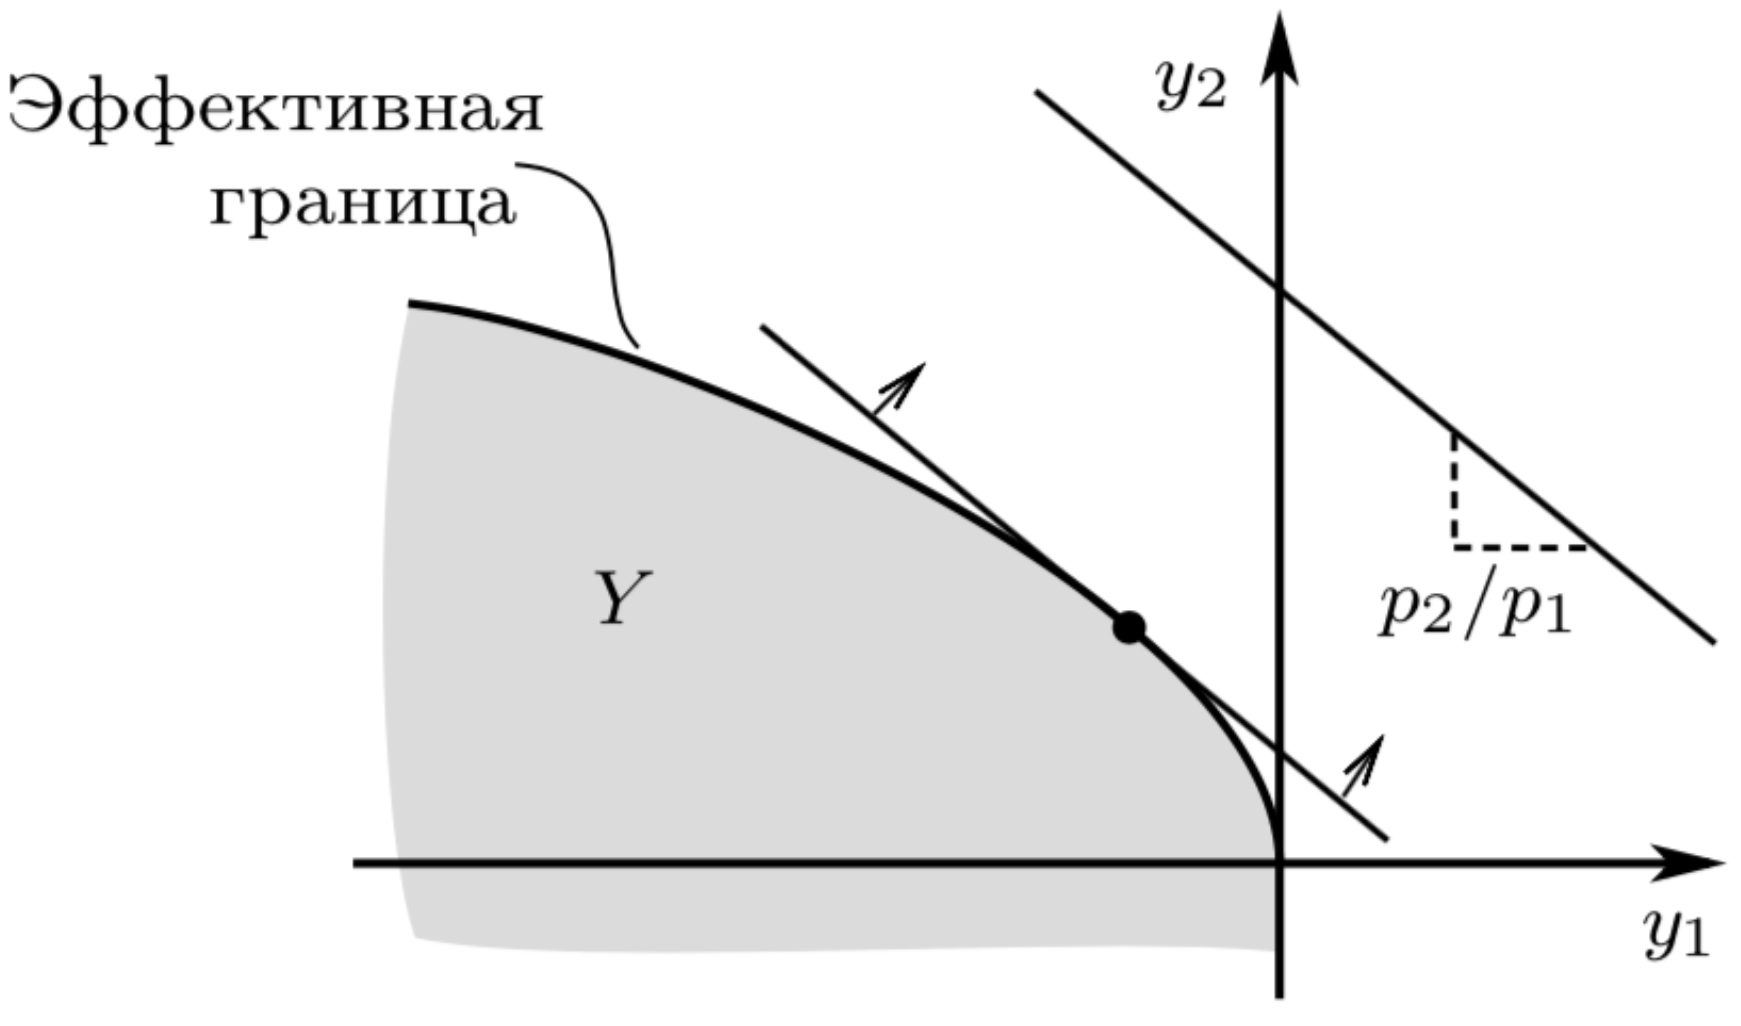
\includegraphics[width=.8 \textwidth]{prod_set.png}
\end{figure}

\end{frame}

\begin{frame}{Технологические множества}

Формально технологическая граница состоит из точек $y \in Y$, таких, что не существует $y' \in Y$, так что $y_i' \geqslant y_i$ по всем координатам $i$ и $y_j' > y_j$ по хотя бы одной координате $j$.

\begin{lemma}
Технологическая граница ищется как все точки $z \in Y$ т.ч.
$$ z \in \text{argmax } \vec q \cdot \vec y, \quad \vec y \in Y,$$
для хотя бы одного вектора цен $\vec q \geqslant 0, \vec q \neq 0$.
\end{lemma}
\end{frame}

\section{Аксиомы производителя}

\begin{frame}{Аксиомы производителя}

Фирма воспринимает технологическое множество и максимизирует прибыль:
$$ \vec q \cdot y \to \max, \quad \vec y \in Y.$$
Чтобы задача была выпуклой, нам понадобятся некоторые аксиомы.

\end{frame}

\begin{frame}{Аксиомы производителя}

\begin{definition}
Аксиомы технологического множества $Y$:

- A1: $Y$ содержит $\vec{0}$
- A2: свобода расходования
$$ y \in Y, y' < y \quad \Rightarrow \quad y' \in Y$$

- A3: невозрастающая отдача от масштаба:
$$y \in Y \Rightarrow \lambda Y \in Y, \quad \forall \lambda \in (0,1)$$

- A4: непусто, замкнуто

- A5: отсутствие рога изобилия: $Y \cap \mathbb{R}^n_{+} = \emptyset$.
\end{definition}

\end{frame}

\begin{frame}{Аксиомы производителя}

Все эти аксиомы нужны, чтобы вывести из них свойства задачи максимизации полезности, которые нам хорошо известны наперед: непрерывность и выпуклость. Гладкость тоже желательна, но, на самом деле, можно обойтись выпуклостью $Y$, поскольку выпуклые функции почти всюду дифференцируемы.

\end{frame}

\begin{frame}{Аксиомы производителя}
\begin{theorem}[БЖЦ]

Если выполнены аксиомы A1-A5, то технологическое множество выпукло. Более того, если производится один товар, то функция $F$, описывающая технологическую границу, непрерывна и вогнута.
\end{theorem}

\end{frame}

\section{Максимизация полезности}

\begin{frame}{Максимизация полезности}
В такой абстрактной постановке удобно анализировать задачу максимизации полезности:
$$ \pi(q, y) = \vec q \cdot \vec y \to \max, \quad y \in Y$$

Как обычно, нас интересуют два объекта:

\begin{itemize}
\item координаты оптимума $y^{\ast}(\vec q)$ - это \textbf{функция предложения}
\item значение целевой функции $\pi^{\ast}(\vec q) = \pi(\vec q, y^{\ast}(\vec q)))$
\end{itemize}

\end{frame}

\begin{frame}{Максимизация полезности}

В такой абстрактной постановке удобно анализировать задачу максимизации полезности:

$$ \pi(q, y) = \vec q \cdot \vec y \to \max, \quad y \in Y$$

Как обычно, нас интересуют два объекта:

\begin{itemize}
\item координаты оптимума $y^{\ast}(\vec q)$ - это абстрактная \alert{функция предложения}
\item значение целевой функции $\pi^{\ast}(\vec q) = \pi(\vec q, y^{\ast}(\vec q)))$
\end{itemize}

Вопрос: В каком пространстве происходит огибание?

Вопрос: Чему равен градиент $\pi^{\ast}(\vec q)$?

Вопрос: Какова форма функции $\pi^{\ast}(\vec q)$?

\end{frame}

\section{Сложение технологических множеств}

\begin{frame}{Сложение технологических множеств}

Предположим, что у нас есть два завода. Первый обладает технологией $Y_1$, второй обладает технологией $Y_2$. Теперь представим себе, что компания владеет этими двумя заводами и может свободно перемещать товары с одного завода на другой и комбинировать любые технологические цепочки. 

Как описать технологическое множество $Y_1 + Y_2$, соответствующее этой компании?

\end{frame}

\begin{frame}{Сложение технологических множеств}

\begin{definition}
Для двух множества $A$ и $B$, их \textbf{евклидова сумма} $A+B$ определяется как:
$$ A+B = \{a + b \ | \ a \in A, \ b \in b\}.$$
\end{definition}
\end{frame}

\begin{frame}{Сложение технологических множеств}
Действительно, компания может <<сложить>> в векторном смысле любые два вектора из множеств $A, B$. 

Первый вектор $a \in A$ означает, что партия товаров была произведена на первом заводе и была отправлена на склад. Второй вектор $b \in B$ означает, что партия товаров была произведена на втором заводе и тоже отправлена на склад. 

На складе партии будут объединены и суммарный объем будет соответствовать вектору $a + b$.
\end{frame}

\begin{frame}{Сложение технологических множеств}
\begin{lemma}
Арифметическая сумма двух выпуклых множеств выпукла.
\end{lemma}
Любая взвешенная сумма двух векторов из $A+B$ представляется как сумма двух взвешенных пар векторов из $A$ и $B$ с теми же весами.
$$ \alpha(a + b) + (1-\alpha)(a'+b') = [\alpha a + (1-\alpha) a'] + [\alpha b + (1-\alpha) b']$$
Соответственно, она тоже лежит в $A + B$.
\end{frame}

\section{Сложение технологических границ}

\begin{frame}{Сложение технологических границ}

Предположим далее, что $Y_1$ описывается производственной функцией $F_1$, а $Y_2$ описывается производственной функцией $F_2$. Как будет выглядеть производственная функция для $Y_1 + Y_2$?

Какие есть кандидаты?
\begin{itemize}
  \item $F_1 + F_2$
  \item $\max(F_1 + F_2)$
  \item $\nabla F_1 = \nabla F_2$
\end{itemize}

\end{frame}

\begin{frame}{Сложение технологических границ}

Легко видеть, что производственная функция $F$ множества $Y_1 + Y_2$ определяется как верхняя огибающая семейства опорных функций: $$F(x_1, \ldots, x_n) : = \max_{\hat x} \left(F_1(\hat x_1, \ldots, \hat x_n) + F_2(x_1 - \hat x_1, \ldots, x_n - \hat x_n)\right),$$

то есть мы сначала решаем сколько произвести на первом заводе, а потом производим остальное на втором заводе. 

Что нам говорит Теорема об Огибающей?

\end{frame}

\begin{frame}{Сложение технологических границ}

$$F(x_1, \ldots, x_n) : = \max_{\hat x} \left(F_1(\hat x_1, \ldots, \hat x_n) + F_2(x_1 - \hat x_1, \ldots, x_n - \hat x_n)\right)$$

Наклон огибающей равен наклону опорной функции в точке касания:
$$ \nabla F = \nabla F_2.$$

\end{frame}

\begin{frame}{Сложение технологических границ}

С другой стороны, можно сказать, что
$$F(x_1, \ldots, x_n) : = \max_{\hat x} \left(F_2(\hat x_1, \ldots, \hat x_n) + F_1(x_1 - \hat x_1, \ldots, x_n - \hat x_n)\right),$$

то есть мы сначала решаем сколько произвести на первом заводе, а потом производим остальное на втором заводе

\end{frame}

\begin{frame}{Сложение технологических границ}

$$F(x_1, \ldots, x_n) : = \max_{\hat x} \left(F_2(\hat x_1, \ldots, \hat x_n) + F_1(x_1 - \hat x_1, \ldots, x_n - \hat x_n)\right)$$

И снова Теорема об Огибающей:
$$ \nabla F = \nabla F_1.$$

\end{frame}

\begin{frame}{Сложение технологических границ}
Получается, что необходимым условием для того, чтобы точка лежала на границе объединенного технологического множества $\vec y \in Y_1 + Y_2$ является то, что, при разложении $\vec y = \vec y_1 + \vec y_2$ этой точки на вектор $\vec y_1 \in Y_1$ и вектор $\vec y_2 \in Y_2$:
$$ \nabla F_1(\vec y_1) =  \nabla F_2(\vec y_2).$$

\end{frame}

\begin{frame}{Сложение технологических границ}
С другой стороны, очевидно, что при разложении $\vec y = \vec y_1 + \vec y_2$ этой точки, $\vec y_1$ на границе $Y_1$, а $\vec y_2$ лежит на границе $Y_2$. 

Таким образом, для того, чтобы описать суммарную технологическую границу, надо сложить только те пары точек $y_1 = F_1(\vec x_1)$ и $y_2 \in F_2(\vec x_2)$, в которых наклоны равны, и сосчитать $(\vec x_1 + \vec x_2, y_1 + y_2)$.

\end{frame}
\section{Сложение треугольников (на доске)}
\section{Конец}

\end{document}